\section{Production Economy}

In this section, we provide some more details on the production economy studied in Section IV.B in the paper. Agents are endowed with capital instead of a Lucas tree. Capital is traded and agents agree on its price. The capital of agents who die is reallocated to the newborn agents. Investors face dynamically complete security markets as in the case of our exchange economy. The dynamics of capital are
\begin{equation}
	dK_t = \left(\psi \left(\iota_t\right) + \mu_K-\delta\right)K_t \:  dt + \sigma_K K_t \: dZ_{K,t}.
\end{equation}
Investments are subject to an adjustment costs represented by the function, $\psi \left(\iota\right) = \frac{log\left(\kappa \iota + 1\right)}{\kappa}$, where $\iota_t$ is the investment rate per unit of capital and $\kappa$ is the investment cost parameter. The second component of the expected growth rate in capital is, $\mu_K-\delta$, where $\mu_K$ represents productivity improvements and $\delta$ is depreciation. One unit of capital produces $a$ units of the consumption good and thus output is $Y_t = a K_t$.\footnote{One can show that all agents will make the same choice, and therefore we do not model the investment choice of each individual agent but instead consider the representative firm.} The resource constraint is $Y_t = C_t + I_t$ where aggregate investment is $I_t=\iota_t K_t$. Let $Q_t$ denote the price of capital which is determined in equilibrium. We posit that the dynamics of $Q_t$ are
\begin{equation}
	dQ_t = Q_t\left(\mu_{Q,t} dt + \sigma^{K}_{Q,t} dZ_{K,t} + \sigma^{\alpha}_{Q,t} dZ_{\alpha,t} \right),
\end{equation}
where the drift, $\mu_{Q,t}$, the supply shock exposure, $\sigma^{K}_{Q,t}$, and the demand shock exposure, $\sigma^{\alpha}_{Q,t}$ will be determined in equilibrium. Given the optimal investment rate, $\iota_t$, the firm pays out $D_t = \left(a-\iota_t\right)K_t$ in dividends and by market clearing we have that $C_t = D_t$. Moreover, the total value of the firm is $S_t = Q_t K_t$ and thus the total return on the stock market is
{\small
\begin{align}
	dR_t &=  \frac{D_t}{S_t}dt + \frac{dS_t}{S_t} = \frac{D_t}{S_t}dt + \frac{dK_t}{K_t}  + \frac{dQ_t}{Q_t} + \frac{dK_t}{K_t} \frac{dQ_t}{Q_t} \nonumber \\
	        &=  \left(\frac{a-\iota_t}{Q_t} + \psi   \left(\iota_t\right)  + \mu_K-\delta + \mu_{Q,t} + \sigma_K \sigma^{K}_{Q,t}\right)dt  
	         + \left(\sigma_K+ \sigma^{K}_{Q,t}\right)dZ_{Y,t} + \sigma^{\alpha}_{Q,t}dZ_{\alpha,t}.
\end{align}
}
To obtain the optimal investment rate, we maximize the value of the firm which is equivalent to 
\begin{equation}\label{IAprodOptInv}
	\underset{\{\iota_t \}}{\max} \quad E [ dR_t].
\end{equation}
state by state. The FOC of the firm's maximization problem in Equation (\ref{IAprodOptInv}) is $\frac{1}{Q_t} = \psi' \left(\iota_t\right)$. Using the expression for the adjustment cost function and solving it for the investment rate, $\iota_t$, we get
\begin{equation}\label{optinv}
	\iota_t = \frac{Q_t - 1}{\kappa}.
\end{equation}
Total wealth in the economy is $S_t = Q_t K_t$ and so the following holds true
\begin{equation}\label{ClearingW}
 \begin{split}	
 	S_t &= Q_t K_t = \int_{-\infty}^t \nu e^{-\nu\left(t-s\right)}\left(\alpha_{s,t}W^a_{s,t} + \left(1-\alpha_{s,t}\right)W^b_{s,t}\right)ds  \\
	&=z  \int_{-\infty}^t \nu e^{-\nu\left(t-s\right)}\left(\alpha_{s,t}\frac{C^a_{s,t}}{\rho_a+\nu} 
	+ \left(1-\alpha_{s,t}\right)\frac{C^b_{s,t}}{\rho_b+\nu}\right)ds   \\
	&=  \left(\frac{f_t}{\rho_a+\nu}+\frac{1-f_t}{\rho_b+\nu}\right)C_t 
	= \left(\frac{f_t}{\rho_a+\nu}+\frac{1-f_t}{\rho_b+\nu}\right)\left(a-\iota_t\right)K_t.
 \end{split}	
\end{equation}
Using Equation (\ref{ClearingW}) and the optimal investment rate from Equation (\ref{optinv}) we have that
\begin{equation}\label{qpart}
	Q_t = \phi_t \left(a-\frac{Q_t}{\kappa} + \frac{1}{\kappa}\right),
\end{equation}
where $\phi_t = S_t/C_t = \mathcal{E}_{f_t}\left(\frac{1}{\rho+\nu}\right)=\left(\frac{f_t}{\rho_a+\nu}+\frac{1-f_t}{\rho_b+\nu}\right)$ is the price-consumption or wealth-consumption ratio, which is the same expression as in the exchange economy, but it is no longer the price-dividend ratio. Solving Equation (\ref{qpart}) for the price of capital we get
\begin{equation}
	Q_t = \frac{1+\kappa a}{1+\kappa \phi_t^{-1}}.
\end{equation}
When the capital adjustment costs approaches infinity, then the optimal investment rate is $\iota_t = 0$,  the price of capital is $Q_t = a \phi_t$, the dividend is $D_t = C_t = aK_t$, and the price-dividend ratio is the same as in the exchange economy, that is, $\frac{S_t}{D_t} = \frac{Q_t K_t}{a K_t} = \frac{a \phi_t}{a} = \phi_t$. 

Adding production to our demand disagreement model does not change how the agents split the ``pie" (output, which is now endogenous). Hence, the consumption share, $f_t$, in the production economy is the same as in the exchange economy with dynamics given by
\begin{equation}
  \begin{split}
	\label{eq:muf}
	\mu_{f,t} &= \nu\left(\alpha_t \beta^a_t \left(1-f_t\right) - \left(1-\alpha_t\right)\beta^b_t f_t\right) + \left(\rho^b-\rho^a\right)f_t\left(1-f_t\right) \\ 
	&+ \Delta^2 \left( \frac{1}{2} - f_t \right) f_t\left(1-f_t\right) 
	\qquad \text{and} \qquad \sigma_{f,t} = f_t (1-f_t) \Delta. 
  \end{split}
\end{equation}
We know from the exchange economy that $\phi_t$ is an affine function of the consumption share $f_t$ hence the dynamics of $\phi_t$ are
\begin{equation}
	\frac{d\phi_t}{\phi_t} = \frac{\phi^a-\phi^b}{\phi_t}\left(\mu_{f,t}dt + \sigma_{f,t}dZ_{\alpha,t}\right).
\end{equation}
Instead of working directly with $\phi_t$, is is useful to define its reciprocal $E_t = \phi_t^{-1}$. The dynamics of $E_t$ are 
\begin{equation}
	dE_t = E_t\left(\mu_{E,t}dt + \sigma_{E,t}dZ_{\alpha,t}\right),
\end{equation}
where 
\begin{align}
	\mu_{E,t} &=  \frac{\phi^a-\phi^b}{\phi_t}\left(\frac{\phi^a-\phi^b}{\phi_t}\sigma_{f,t}^2 - \mu_{f,t}\right) \\
	\sigma_{E,t} &=   -\frac{\phi^a-\phi^b}{\phi_t}\sigma_{f,t}.
\end{align}
Using the definition of $E_t$ we we get for the price of capital $Q_t = Q\left(E_t\right) = \frac{1+a \kappa}{1+\kappa E_t}$. Hence, by It\^o's lemma 
\begin{align}
	\mu_{Q,t} &= w_t^2 \sigma_{E,t}^2 - w_t \mu_{E,t} \\
	\sigma^{K}_{Q,t} &=  0 \\
	\sigma^{\alpha}_{Q,t} &=  -w_t \sigma_{E,t},   
\end{align}
where $w_t = \frac{\kappa E_t}{1+\kappa E_t}$ with $0 \leq w_t \leq 1$. Since, $S_t = Q_t K_t$ it immediately follows that stock market loadings onto the shocks are given by
\begin{align}
	\sigma^K_{S,t} &=  \sigma_K \\
	\sigma^{\alpha}_{S,t} &=  -w_t \sigma_{E,t} = w_t  \frac{\phi^a-\phi^b}{\phi_t}\sigma_{f,t}. \label{stockmarketloading}
\end{align}
Consequently,  the stock market loading on the demand shock is is the same as in the exchange economy multiplied by the weight $w_t$. Next, we determine the dynamics of aggregate consumption. First note that the investment rate, $\iota_t = \frac{Q_t-1}{\kappa}$ has dynamics
\begin{equation}
	d\iota_t = \mu_{\iota,t}dt + \sigma_{\iota,t}dZ_{\alpha,t}.
\end{equation}
where $ \mu_{\iota,t} = \frac{1}{\kappa}Q_t\mu_{Q,t}$ and $\sigma_{\iota,t} = \frac{1}{\kappa}Q_t \sigma^{\alpha}_{Q,t}$. Aggregate consumption equals  $C_t = \left(a-\iota_t\right)K_t$ and so applying Ito's lemma yields
\begin{equation}
	dC_t = C_t \left(\mu_{C,t}dt + \sigma^{K}_{C,t}dZ_{Y,t} + \sigma^{\alpha}_{C,t}dZ_{\alpha,t}\right),
\end{equation}
where 
\begin{align}
	\mu_{C,t} &=   \psi \left(\iota_t\right) + \mu_K-\delta - \frac{1}{a-\iota_t}\mu_{\iota,t} \\
	\sigma^{K}_{C,t} &= \sigma_K \\
	 \sigma^{\alpha}_{C,t} &=  -\frac{\phi_t}{\kappa+\phi_t} \frac{\phi^a-\phi^b}{\phi_t}\sigma_{f,t}  \label{diffusionC}
\end{align}
Comparing the diffusion in Equation (\ref{diffusionC}) with the stock market loading on the demand shock in Equation (\ref{stockmarketloading}) we see that it has the opposite sign. Hence, good news for the stock market is bad news for consumption growth. To derive the stochastic discount factor, we have (just as in the exchange economy) that $\xi_t = \frac{X_t}{C_t}$ where $X_t$ satisfy the following integral equation
\begin{equation}
	X_t = \int_{-\infty}^{t}\nu e^{-\nu\left(t-s\right)}\left(\alpha_s \beta^a_s e^{-\rho_a \left(t-s\right)}\frac{\eta^a_t}{\eta^a_s}+(1-\alpha_s) \beta^b_s e^{-\rho_b \left(t-s\right)}\frac{\eta^a_t}{\eta^a_s}\right)X_s ds.
\end{equation}
Applying Ito's lemma to $\xi_t = \frac{X_t}{C_t}$ leads to the dynamics of the SDF and hence the risk-free rate is
\begin{align}
	r_t &=  \rho_a f_t + \rho_b \left(1-f_t\right) + \mu_{C,t} - \sigma_{K}^2  - \left(\sigma^{\alpha}_{C,t}\right)^2 \\
	&  + \sigma^{\alpha}_C\Delta\left(\frac{1}{2}-f_t\right)   
	   + \nu\left(1-\alpha_t \beta^a_t - \left(1-\alpha_t\right)\beta^b_t\right) 
\end{align}
and the market price of supply and demand shock risk are
\begin{align}
	\theta_{K,t} &=  \sigma_{K} \\
	\theta_{\alpha,t} &=  \sigma^{\alpha}_{C,t} + \Delta\left(\frac{1}{2}-f_t\right),
\end{align}
respectively. In contrast to the exchange economy, the risk-free rate now depends directly on the disagreement $\Delta$ and the market price of demand shock risk depends on the consumption loading on demand shocks. 

The lower right graph of Figure \ref{fig:prod} shows the unconditional mean of the  demand shock exposure of aggregate consumption, $\sigma^{\alpha}_{C,t}$ as a function of the adjustment cost parameter $\kappa$. Importantly, the demand shock exposure is negative and approaches zero as we increase $\kappa$ because a demand shock increases the consumption share of patient investors and thus lowers the discount rate. A lower discount rate increases investment, but as aggregate output has no exposure to demand shocks this increase comes at the expense of lower consumption growth. 
\begin{figure}[htbp] 
\centering
\vspace{0.1in}
\begin{tabular}{ccc}
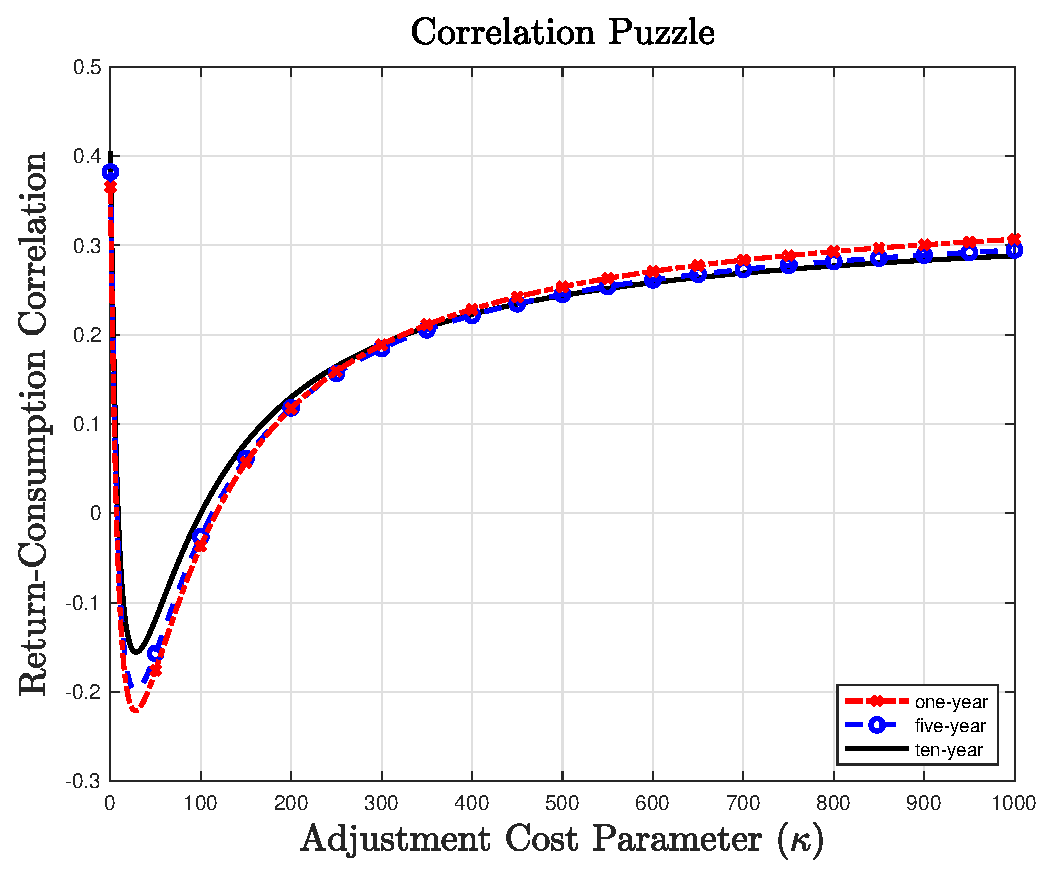
\includegraphics[width=.3\textwidth]{figures/FigProdCorrpuzzle.eps} &
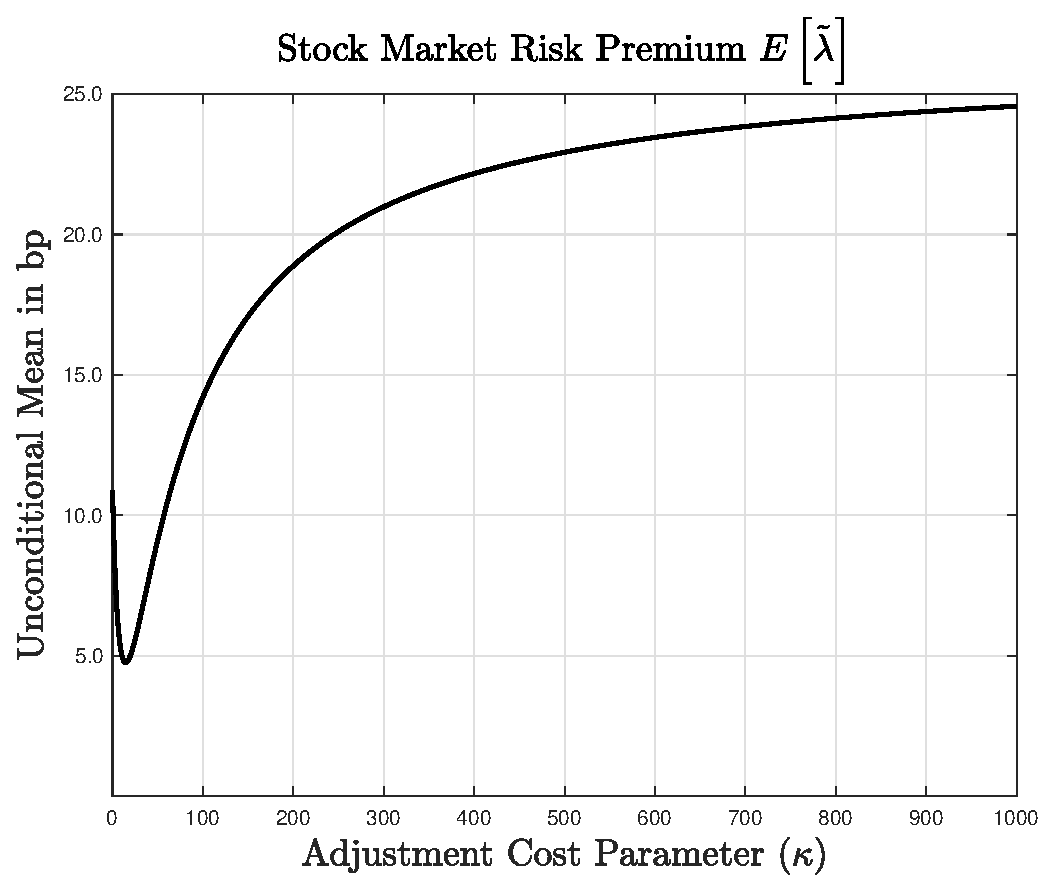
\includegraphics[width=.3\textwidth]{figures/FigProdRP.eps} &
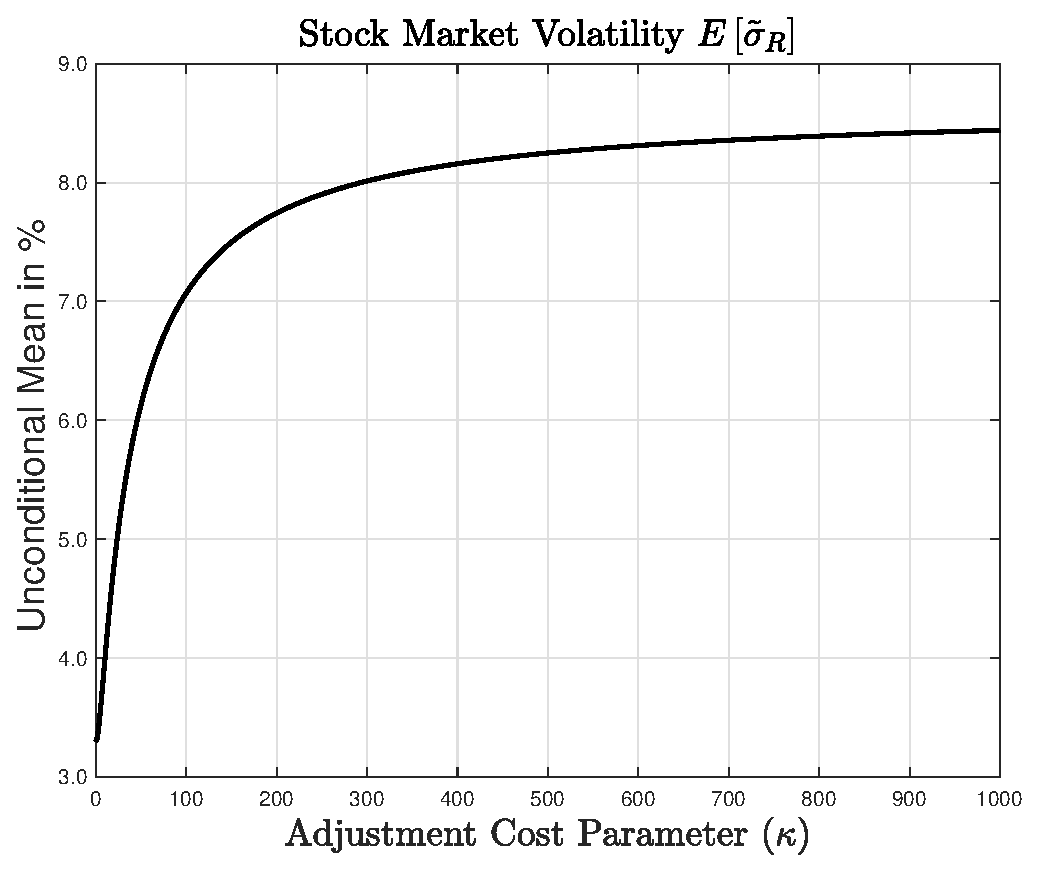
\includegraphics[width=.3\textwidth]{figures/FigProdStdevS.eps}  \\
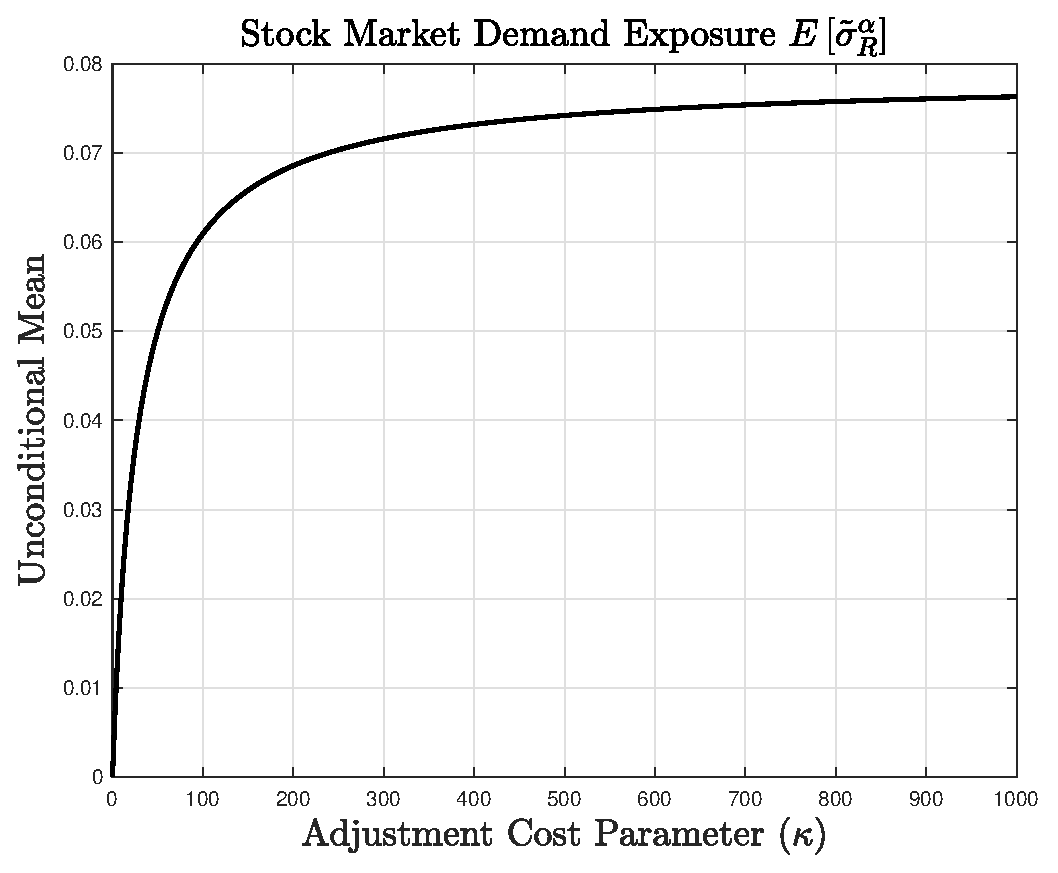
\includegraphics[width=.3\textwidth]{figures/FigProdsigalpS.eps}  &
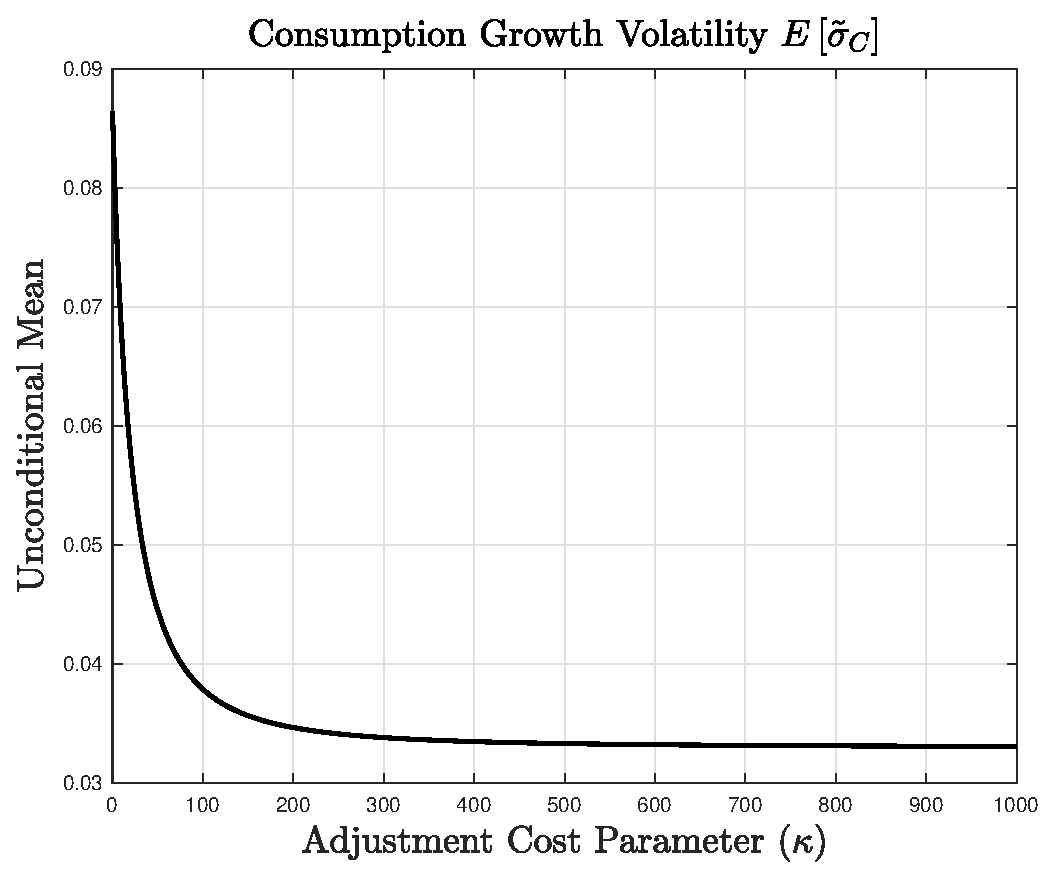
\includegraphics[width=.3\textwidth]{figures/FigProdStdevC.eps} &
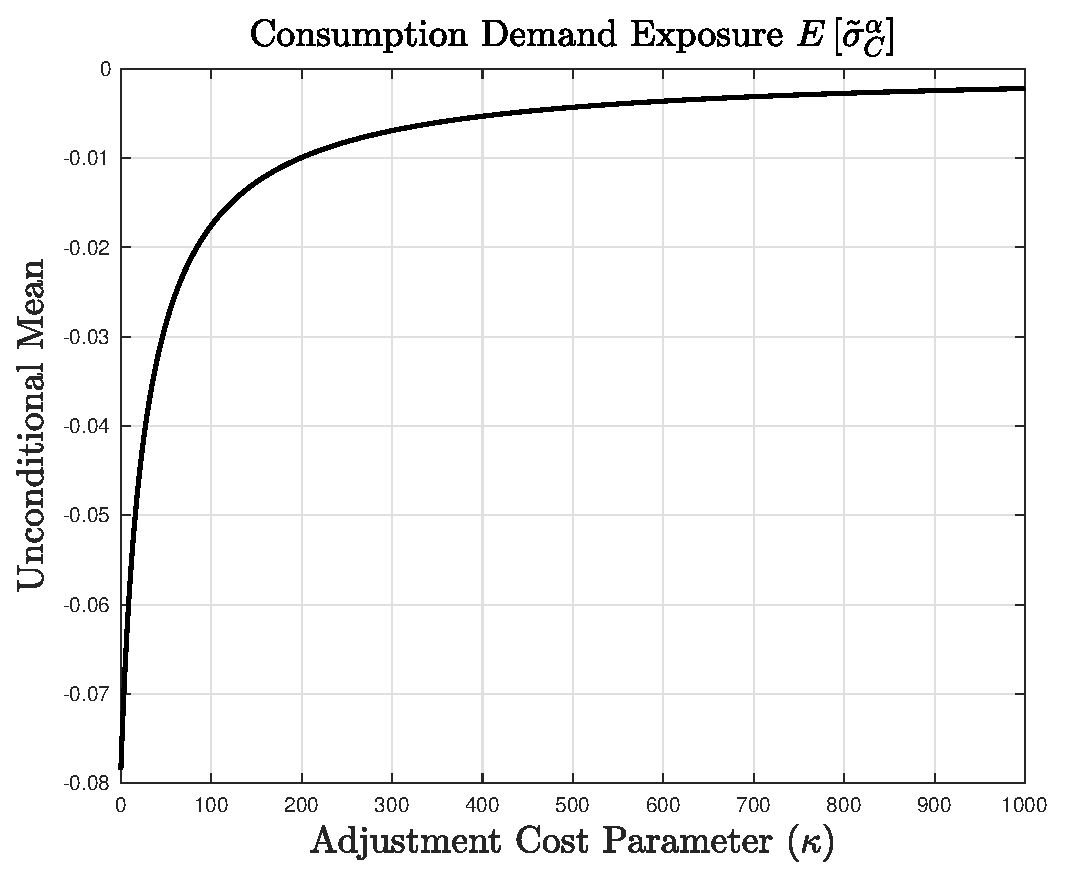
\includegraphics[width=.3\textwidth]{figures/FigProdsigalpC.eps} 
\end{tabular}
\caption{\emph{Demand disagreement in a production model.} \footnotesize{The graphs show the unconditional mean of the return-consumption correlation, the stock market risk premium, the stock market volatility, the stock market demand exposure, the consumption growth volatility, and the consumption demand exposure as a function of the adjustment cost parameter $\kappa$. The summary statistics are based on one million years of monthly observations for each value of $\kappa$.}} \label{fig:prod}
\end{figure}

In contrast to consumption, demand shocks are good news for the stock markets as they lower discount rates. Hence, the unconditional mean of the stock market's exposure to demand shocks is positive as in the exchange economy which we show with the bottom left graph of Figure \ref{fig:prod}. While both consumption growth and stock returns have the same exposure to the productivity of capital they have different exposure to demand shocks. The top left graph shows that this leads to a low correlation between stock returns and consumption growth, that in contrast to an exchange economy, may even be negative. Interestingly, the risk premium for demand shocks is still positive even though aggregate consumption loads negatively on them. The intuition is the same as in the baseline model with the exception that the negative loading partly offsets it. However, it is not strong enough to completely offset the effect, and therefore the risk premium is positive. 


	
	



